\section{Implementación}

Debido a la extensión del proyecto no se llegó a diseñar el circuito en su totalidad,
por lo que solo se implementó el convertidor de tensión continua
junto con el generador de señal PWM y el driver.

El objetivo mínimo propuesto es el diseño y construcción de la primera etapa de la fuente de switching. 
Se deben obtener las señales de tensión y corriente sobre los elementos operando a lazo abierto con un ciclo de trabajo fijo. 

Se construyó un prototipo funcional para cumplir con las especificaciones propuestas. 
Debido a que el costo de una batería de litio de las características necesarias es elevado,
se redujo la tensión de salida a $12.6V$, tensión que normalmente se utiliza para recargar baterías de computadoras portátiles.

Para una mayor seguridad se optó por reemplazar la primera etapa de conversión AC-DC por una fuente regulable cuya tensión de entrada sea de $36V$.
Las primeras pruebas se realizaron en una placa de cobre perforada y las mediciones finales se realizaron sobre un circuito impreso. 

A continuación se detalla el instrumental utilizado para alimentar al circuito y realizar las mediciones necesarias:

\begin{itemize}
    \item Dos fuentes regulables. La primera de ellas se ajustó en $12V$ para alimentar al TL494, y la segunda es una fuente partida de $\pm18V$ que se estableció en $36V$. Las fuentes tienen una corriente máxima de $1A$.
    \item Multímetros para la medición de corriente y tensión de salida. 
    \item Un osciloscopio para obtener las señales de tensión y corriente en cada componente.
    \item Una resistencia de carga de $10k\Omega$ y $71W$. 
\end{itemize}

\begin{figure}[H]
    \centering
    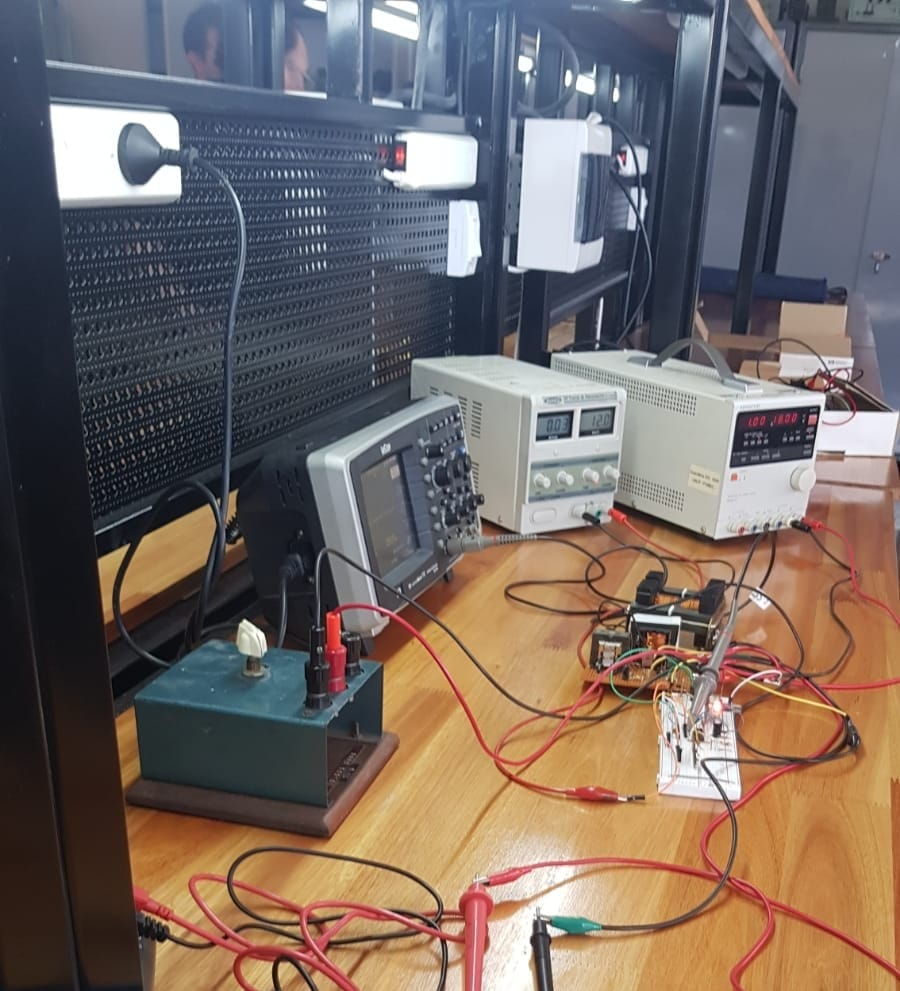
\includegraphics[width=0.6\textwidth]{images/setup.jpeg}
    \caption{Banco de pruebas armado en el ATEI.}
    \label{fig:setup}
\end{figure}